\clearpage
\clearpage
\begin{center}
    \textbf{\Large Supplementary Materials: Learning Deeply Enriched Representations of Longitudinal Imaging-Genetic Data to Predict Alzheimer's Disease Progression}
\end{center}
\beginsupplement

\section{Perturbation Based Biomarker Identification}
For the longitudinal records of $q$-th biomarker ($1 \leq q \leq D_l$) and $i$-th participant, we sample the column vector of perturbations $\mathbf{p}_{i,q} \in \Re^{n_i}$ from the normal distribution $\mathcal{N}(0, \sigma_q^2)$ with zero mean and the same standard deviation as the observed distribution of $q$-th biomarker across all $n$ participants, and add the perturbation to the records as follows:
\begin{equation}
\begin{aligned}
    &N = \sum_{i=1}^n \sum_{j=1}^{n_i} \sum_{q=1}^{D_l} [\mathbf{M}_i]^j_q,\ \mu_q = \frac{1}{N}\sum_{i=1}^n \sum_{j=1}^{n_i} \sum_{q=1}^{D_l} [\mathbf{X}_i \odot \mathbf{M}_i]^j_q,\ \sigma_q^2 = \frac{1}{N}\sum_{i=1}^n \sum_{j=1}^{n_i} \sum_{q=1}^{D_l}\\
    &[\mathbf{M}_i]^j_q ([\mathbf{X}_i]^j_q - \mu_q)^2,\ \mathbf{X}_i' = [[\mathbf{X}_i]_1, [\mathbf{X}_i]_2, \cdots, [\mathbf{X}_i]_q + \mathbf{p}_{i, q}, \cdots, [\mathbf{X}_i]_{D_l}].
\end{aligned}
\end{equation}
Then the prediction changes by the perturbation are:
\begin{equation}\label{eq: neuroimaging identification}
\begin{aligned}
    &\Delta\tilde{\mathbf{y}}_i = \| \psi_{pred}\bigl(\phi_{dynamic}(\mathbf{X}_i', \mathbf{M}_i, \mathbf{t}_i;\ \theta_{\phi}^l),\ \psi_{SNP}(\phi_{SNP}(\mathbf{x}_i^s;\ \theta^s_{\phi});\ \theta^s_{\psi}),\ \mathbf{x}_i^b;\ \theta^p_{\psi}\bigr)\\
    &- \psi_{pred}\bigl(\phi_{dynamic}(\mathbf{X}_i, \mathbf{M}_i, \mathbf{t}_i;\ \theta_{\phi}^l),\ \psi_{SNP}(\phi_{SNP}(\mathbf{x}_i^s;\ \theta^s_{\phi});\ \theta^s_{\psi}),\ \mathbf{x}_i^b;\ \theta^p_{\psi}\bigr)\|_1.
\end{aligned}
\end{equation}
The importance of $q$-th biomarker is the average of prediction changes across all the participants: $\frac{1}{n}\sum_{i=1}^n\Delta\tilde{\mathbf{y}}_i$. Similarly, we can calculate the input genetic data whose $q$-th SNP is perturbed and it's prediction changes.

\section{Hyperparameters of proposed model}
For our model, semi-supervised autoencoder (SAE), the static encoder $\phi_{SNP}$ and decoder $\psi_{SNP}$ have 2 fully connected layers (FC) each with the tanh activation function at the first to third layer and logistic sigmoid at the fourth layer. The dynamic decoder $\psi_{dynamic}$ has 3 FCs with a leaky rectified linear unit (alpha = 0.1) activation function at the first layer and tanh at the second and third layer. The dynamic encoder $\phi_{dynamic}$ is the LSTM with 64 units and tanh activation function. We set $\gamma_1 = 1e+2$, $\gamma_2 = 1e+1$, $\gamma_3 = 1$ in Eq.~\eqref{eq: total loss}.
To minimize the loss function in Eq.~\eqref{eq: total loss}, we adapt the Adam optimizer~\cite{kingma2014adam} at a fixed learning rate of 0.0003 and the other parameters are kept at their default values. We do not use any regularization or dropout techniques, as they degrade the performance.

% \section{Definitions of Evaluation Metrics}
% \begin{equation}\label{eq: metrics}
%     \begin{aligned}
%         &\text{Accuracy} = \frac{\sum_{c \in C}(TP_c + TN_c)}{\sum_{c \in C}(TP_c + TN_c + FP_c + FN_c)},\\
%         &\text{Precision of class }c=\frac{TP_c}{TP_c + FP_c},\ \text{Recall of class }c=\frac{TP_c}{TP_c+FN_c},
% \end{aligned}
% \end{equation}
% where $C$ is a set of classes \{AD, MCI, HC\}.

\begin{figure}
    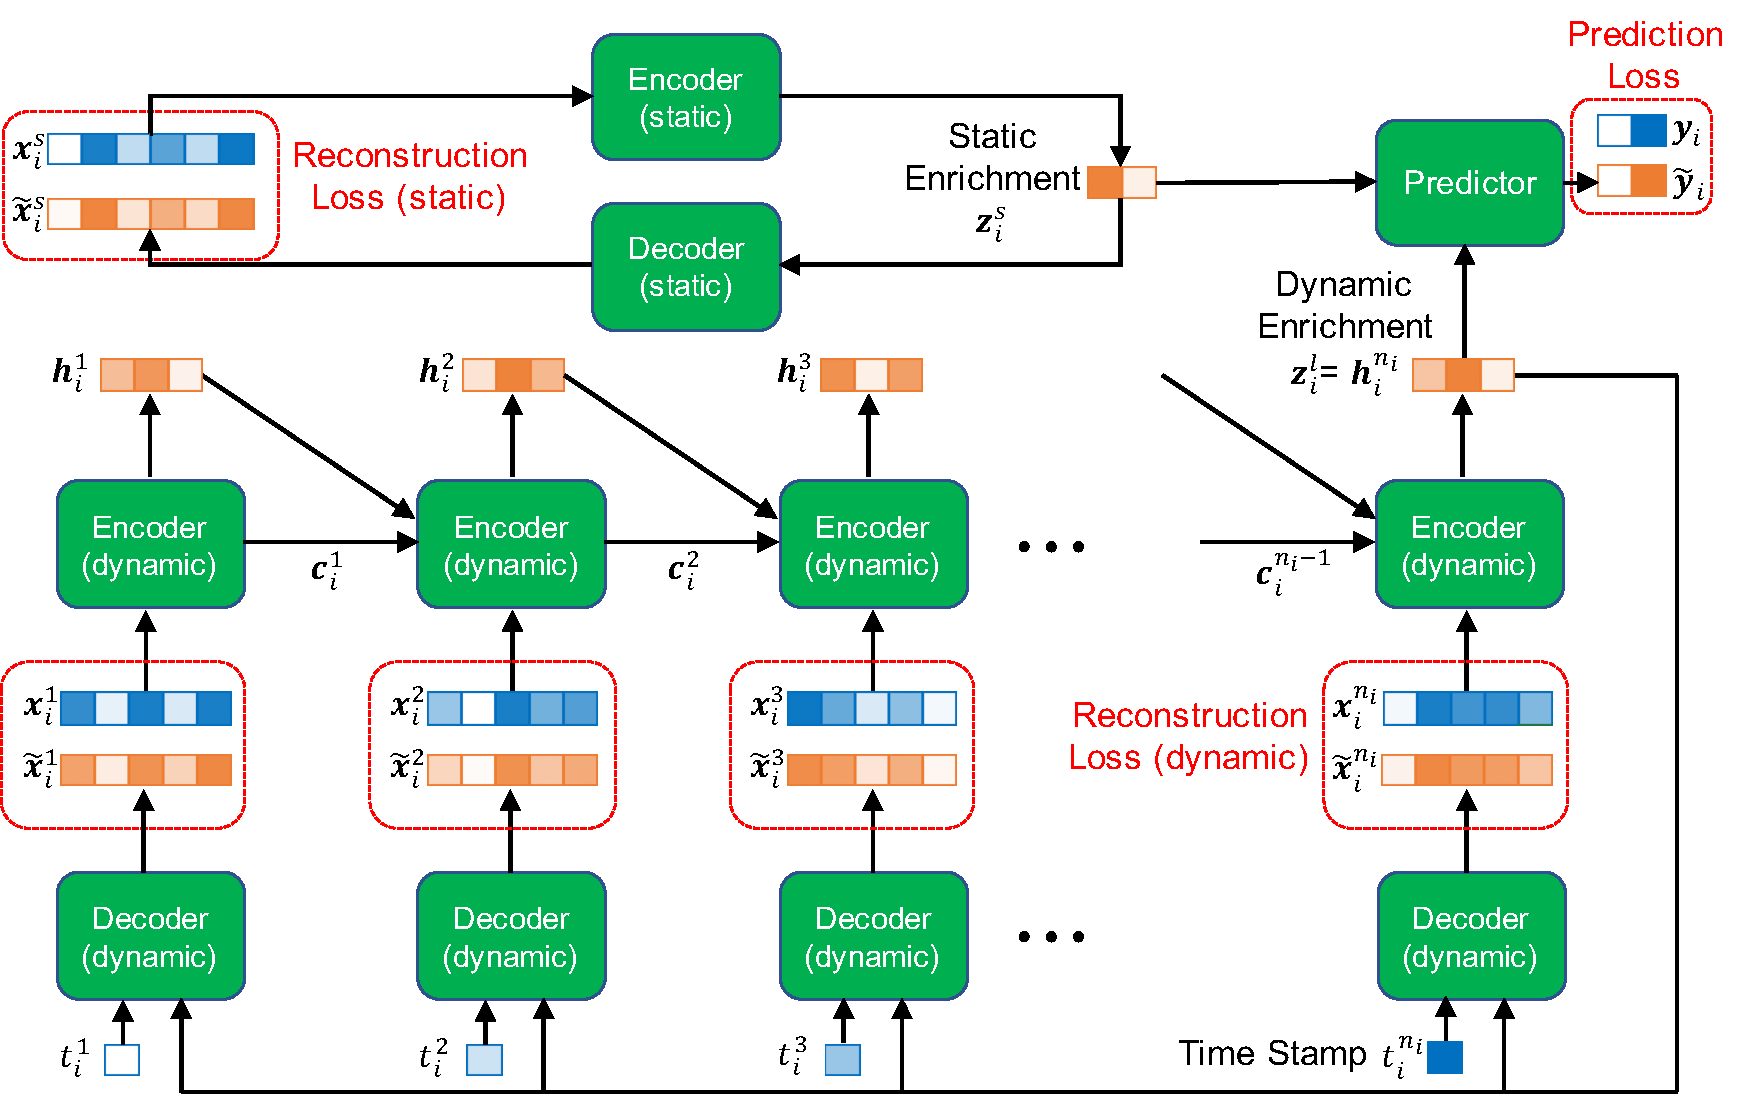
\includegraphics[width=\textwidth]{images/objective.pdf}
    \caption{An schematic illustration about loss function. Our semi-supervised learning autoencoder minimizes the reconstruction loss for the labeled or unlabeled samples, and prediction loss only for the labeled samples.} \label{fig: objective}
\end{figure}

\begin{figure}
    \centering
    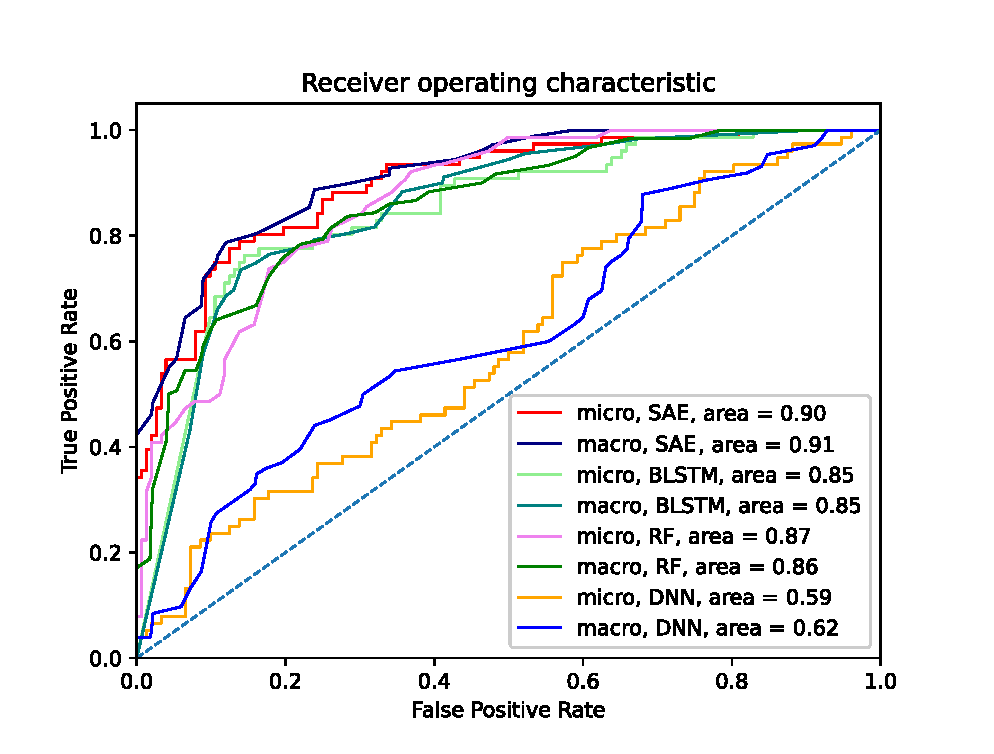
\includegraphics[width=0.89\textwidth]{images/roc_curve-p8.eps}
    \caption{Micro and macro receiver operating characteristic curves (ROC) averaged across the classes and their area under the curve (AUC). The proportion of training set is 80\% and the AUC shows SAE outperforms the other competing models.} \label{fig: roc_curve}
\end{figure}